\documentclass[12pt,letterpaper]{article}
\usepackage{amsmath}
\usepackage{amsfonts}
\usepackage{amsthm}
\usepackage{cancel}
\usepackage[margin=1in]{geometry}
\usepackage{titling}
\usepackage{graphicx}

\setlength{\droptitle}{-10ex}

\preauthor{\begin{flushright}\large \lineskip 0.5em}
\postauthor{\par\end{flushright}}
\predate{\begin{flushright}\large}
\postdate{\par\end{flushright}}

\title{ECS 170 Homework 3\vspace{-2ex}}
\author{Hardy Jones\\
        999397426\\
        Professor Davidson\vspace{-2ex}}
\date{Winter 2014}

\begin{document}
  \maketitle

  \begin{enumerate}
    \item
      We discussed the $\alpha-\beta$ pruning technique for improving the runtime of the minimax algorithm.
      Given a game tree with maximum depth $m$, branching factor $b$, and minimum depth of an optimal state $d$:

      \begin{enumerate}
        \item What is the worst case runtime?

          The worst case runtime is $O(b^m)$.
        \item What is the best case runtime?

          The best case runtime is $O(b^\frac{m}{2})$
        \item Under what condition can we achieve best case runtime?

          The best case can be achieved if we examine the best successors first.
      \end{enumerate}
    \item
      Consider the following min-max game tree.

      \begin{enumerate}
        \item
          Execute $\alpha-\beta$ pruning on the example.
          First, write the minimax value at each node.
          Then cross out the branches that get pruned by $\alpha-\beta$ pruning.
          If a branch does get pruned, circle the nodes under that branch that you had to explore in order to decide to prune the branch.

          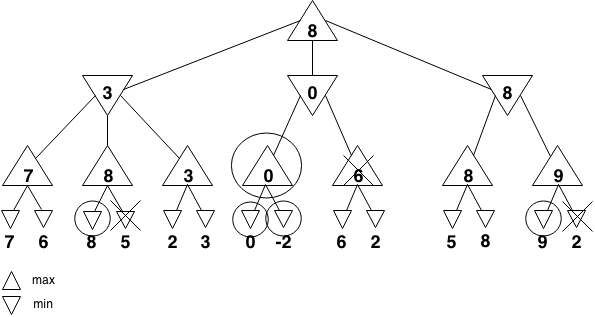
\includegraphics[width=5.5in]{minimax_circled.png}

        \item
          How would you reorder the first moves that max can make
          in order to maximize the number of nodes pruned by $\alpha-\beta$ pruning?
          Assume all other nodes are still expanded from left to right.

          The idea is to have each player enumerate their best moves first.
          This means max wants the largest node in the leftmost subtree,
          while min wants the smallest node in the leftmost subtree.
          Since max makes the final play, we order the nodes according to max's wants rather than min's wants.

          One possible ordering is: [8, 2, 8, 6, 9, 7, 3, 2, 5, 2, 0, -2, 6, 6]
      \end{enumerate}

    \item
      Consider the empty min-max game tree.

      Give a set of minimax values at the leaves such that
      $\alpha-\beta$ pruning will not be able to prune any branches at all.

      The idea here is the opposite of the last question.
      To prevent pruning, we want the worst values to be enumerated by each player.

      One possible ordering is: [6, 7, 2, 6, -2, 0, 2, 5, 2, 3, 8, 9, 6, 8]
  \end{enumerate}
\end{document}
